\documentclass{article}
\usepackage{amsthm,amsmath,amsfonts,lipsum}
\usepackage[T1]{fontenc}
\usepackage{beramono}
\usepackage{listings}
\usepackage{fontawesome5}
\usepackage{adjustbox}
\usepackage{mathabx}
\usepackage{thmtools}
\usepackage{import}
\usepackage{graphicx}
\usepackage{setspace}
\usepackage{geometry}
\usepackage{physics}
\usepackage{float}
\usepackage[english]{babel}
\usepackage{framed}
\usepackage[dvipsnames,x11names]{xcolor}
\usepackage{tcolorbox}
\usepackage{fancyhdr}
\usepackage{hyperref}
\usepackage{booktabs}
\usepackage{enumitem}
\usepackage{cancel}
\usepackage{background}
\usepackage{units}
\usepackage{textcomp}

% Configuring the background
\backgroundsetup{
  scale=1, % Optional, scale if needed
  color=black, % Optional, set the image color, can be omitted
  opacity=0.18, % Optional, adjust opacity for watermark effect
  angle=0,
  position=current page.center, % Center the image on the page
  contents={
\includegraphics[width=1.75\paperwidth, height=1.75\paperheight, keepaspectratio]{ninym_ralei_leaf (watermarked by AlexanderTheMango)}} % Keeps aspect ratio and scales to fill the page
}

% Colours
\definecolor{darkgreen}{rgb}{0.0, 0.5, 0.0}
\definecolor{Firebrick}{rgb}{0.698, 0.132, 0.203}
\definecolor{Crimson}{rgb}{0.862745, 0.078431, 0.235294} % Crimson color
\definecolor{lightred}{rgb}{1.0, 0.819608, 0.819608} % Light red for background
\definecolor{MediumPurple}{rgb}{0.576, 0.439, 0.859}
\definecolor{chocolate}{rgb}{0.82, 0.41, 0.12} % Chocolate color definition
\definecolor{myframecolor}{rgb}{0.25, 0.41, 0.88} % RoyalBlue
\definecolor{mybackgroundcolor}{rgb}{0.68, 0.85, 0.90} % LightSkyBlue
% Define the Navy color
\definecolor{Navy}{rgb}{0.0, 0.0, 0.5}

% Define custom tcolorbox styles for notes
\tcbuselibrary{skins, breakable}
\newtcolorbox{definitionbox}{colframe=RoyalBlue, colback=blue!5!white, title=Definition}
\newtcolorbox{examplebox}{colframe=ForestGreen, colback=green!5!white, title=Example}
\newtcolorbox{notebox}{colframe=RedOrange, colback=orange!5!white, title=Note}
\newtcolorbox{theorembox}{colframe=RoyalPurple, colback=purple!5!white, title=Theorem}

\newtcolorbox{propositionbox}{colframe=myframecolor, colback=mybackgroundcolor!20!white, title=Proposition}
\newtcolorbox{remarkbox}{colframe=MidnightBlue, colback=blue!10!white, title=Remark}
\newtcolorbox{corollarybox}{colframe=OliveGreen, colback=green!10!white, title=Corollary}
\newtcolorbox{warningbox}{colframe=Crimson, colback=lightred, title=Warning}
\newtcolorbox{proofbox}{colframe=Black, colback=gray!10!white, title=Proof}
\newtcolorbox{questionbox}{colframe=Teal, colback=teal!10!white, title=Question}
\newtcolorbox{tipbox}{colframe=Goldenrod, colback=yellow!10!white, title=Tip}
\newtcolorbox{exercisebox}{colframe=darkgreen, colback=green!5!white, title=Exercise}
\newtcolorbox{solutionbox}{colframe=DodgerBlue4, colback=blue!5!white, title=Solution}
\newtcolorbox{algorithmbox}{colframe=Navy, colback=blue!10!white, title=Algorithm}
\newtcolorbox{conceptbox}{colframe=chocolate, colback=brown!10!white, title=Concept}
\newtcolorbox{illustrationbox}{colframe=Firebrick, colback=red!10!white, title=Illustration}
\newtcolorbox{intuitionbox}{colframe=MediumPurple, colback=purple!10!white, title=Intuition}
\newtcolorbox{answerbox}{colframe=RoyalBlue, colback=blue!10!white, title=Answer}

% Geometry settings
\geometry{letterpaper, portrait, includeheadfoot=true, hmargin=1in, vmargin=1in}
\onehalfspacing

% Header and footer
\pagestyle{fancy}
\fancyhf{}
\lhead{MAT232 - Lecture Notes}
\rhead{\thepage}
\lfoot{University of Toronto Mississauga}
\rfoot{\today}

% Document starts
\begin{document}
\renewcommand{\familydefault}{\rmdefault}

\begin{titlepage}
    \null % This is a TeX command that does nothing but is necessary for vfill to work correctly
    \vfill
    \begin{center}
        {\fontsize{40}{48}\selectfont \bfseries MAT232 - Lecture 13}
        \vspace{20pt} \\
        {\LARGE after partial derivatives?} \\
        \vspace{20pt}
        \textbf{AlexanderTheMango}
        \vspace{8pt}
        \\ Prepared for February 24, 2025
    \end{center}
    \vfill
\end{titlepage}


\newpage
\setcounter{page}{0}
\tableofcontents
\newpage

\begin{titlepage}
    \null % Ensures proper alignment with vfill
    \vfill
    \begin{center}
        {\Huge \textbf{Definitions and Theorems}} \\[20pt]
        \rule{\textwidth}{0.5mm} \\[15pt]
        {\Large \textit{Straight from the textbook — lots of fluff this time, more than what we need!}} \\[15pt]
        \rule{\textwidth}{0.5mm} \\[15pt]
        \textbf{Quick recap before diving into the lecture.}
    \end{center}
    \vfill
\end{titlepage}


\section*{Polar Coordinates - Key Theorems}
\addcontentsline{toc}{section}{Polar Coordinates - Key Theorems}

\subsection*{Converting Points between Coordinate Systems}
\addcontentsline{toc}{subsection}{Converting Points between Coordinate Systems}
\begin{theorembox}
    Given a point \( P \) in the plane with Cartesian coordinates \( (x,y) \) and polar coordinates \( (r,\theta) \), the following conversion formulas hold true:
    \[
    x = r \cos\theta \quad \text{and} \quad y = r \sin\theta,
    \]
    \[
    r^2 = x^2 + y^2 \quad \text{and} \quad \tan\theta = \frac{y}{x}.
    \]
    These formulas can be used to convert between rectangular and polar coordinates.
\end{theorembox}

\subsection*{Uniqueness of Polar Coordinates}
\addcontentsline{toc}{subsection}{Uniqueness of Polar Coordinates}
\begin{propositionbox}
    Every point in the plane has an infinite number of representations in polar coordinates. Specifically, the polar coordinates \( (r, \theta) \) of a point are not unique.
    
    \begin{remarkbox}
        For example, the polar coordinates \( (2, \pi/3) \) and \( (2, 7\pi/3) \) both represent the same point in the rectangular coordinate system. Additionally, the value of \( r \) can be negative. Therefore, the point with polar coordinates \( (-2, 4\pi/3) \) represents the same rectangular point as \( (2, \pi/3) \).
    \end{remarkbox}
\end{propositionbox}

\subsection*{Symmetry of Polar Curves}
\addcontentsline{toc}{subsection}{Symmetry of Polar Curves}
\begin{theorembox}
    Polar curves can exhibit symmetry similar to those in rectangular coordinates. The key symmetries to identify are:
    \begin{itemize}
        \item \textbf{Symmetry with respect to the polar axis:} A curve is symmetric with respect to the polar axis if replacing \( \theta \) with \( -\theta \) in its equation yields the same curve.
        \item \textbf{Symmetry with respect to the line \( \theta = \frac{\pi}{2} \):} A curve is symmetric with respect to the line \( \theta = \frac{\pi}{2} \) if replacing \( \theta \) with \( \pi - \theta \) yields the same curve.
        \item \textbf{Symmetry with respect to the pole (origin):} A curve is symmetric with respect to the pole if replacing \( r \) with \( -r \) yields the same curve.
    \end{itemize}
\end{theorembox}

\begin{titlepage}
    \null % Ensures proper alignment with vfill
    \vfill
    \begin{center}
        {\Huge \textbf{Let’s Get Started}} \\[20pt]
        \rule{\textwidth}{0.5mm} \\[15pt]
        {\Large \textit{Time to dive into the lecture notes.}} \\[15pt]
        \rule{\textwidth}{0.5mm} \\[15pt]
        \textbf{Grab your pen or pencil, and let’s break this down step by step.}
    \end{center}
    \vfill
\end{titlepage}

\setcounter{page}{2}
\normalsize

\section*{Plotting Polar Coordinates}
\addcontentsline{toc}{section}{Plotting Polar Coordinates}

\subsection*{Recall the Content from Last Lecture}
\addcontentsline{toc}{subsection}{Recall the Content from Last Lecture}
\begin{notebox}
Converting between Cartesian coordinates \( (x, y) \) and Polar coordinates \( (r, \theta) \):

\begin{algorithmbox}
    \textbf{From Cartesian to Polar:}
    \[
        r = \sqrt{x^2 + y^2}, \quad \theta = \arctan\left(\frac{y}{x}\right)
    \]
    
    \textbf{From Polar to Cartesian:}
    \[
        x = r\cos\theta, \quad y = r\sin\theta
    \]
\end{algorithmbox}

\textbf{Converting Between Degrees and Radians:}
\begin{algorithmbox}
    \begin{itemize}
        \item \textbf{Degrees to Radians:} Multiply by \( \dfrac{\pi}{180^{\circ}} \)
        \[
        \text{Radians} = \text{Degrees} \times \dfrac{\pi}{180^\circ}
        \]
        \item \textbf{Radians to Degrees:} Multiply by \( \dfrac{180^\circ}{\pi} \)
        \[
        \text{Degrees} = \text{Radians} \times \dfrac{180^\circ}{\pi}
        \]
    \end{itemize}
\end{algorithmbox}
\end{notebox}

\subsection*{Understanding the Convention for \( r \) in Polar Coordinates}
\addcontentsline{toc}{subsection}{Understanding the Convention for \( r \) in Polar Coordinates}

\begin{conceptbox}
In polar coordinates, a point is represented as \( (r, \theta) \), where:
\begin{itemize}
    \item \( r \) is the radial distance from the origin (how far the point is from the origin).
    \item \( \theta \) is the angle, measured counterclockwise from the positive x-axis.
\end{itemize}

\begin{notebox}
    \subsubsection*{Special Case: When \( r \) is Negative}
    \begin{itemize}
        \item A negative \( r \) in \( (-r, \theta) \) is interpreted as the point being reflected through the origin.
        \item The equivalent representation is:
        \[
        (-r, \theta) = (r, \theta + 180^\circ)
        \]
        or in radians:
        \[
        (-r, \theta) = (r, \theta + \pi)
        \]
    \end{itemize}
\end{notebox}

\begin{intuitionbox}
    \begin{itemize}
        \item Reflecting \( (r, \theta) \) through the origin is the same as rotating the point by \( 180^\circ \) (or \( \pi \) radians).
        \item This property simplifies polar plots by offering alternate representations of the same point.
    \end{itemize}
\end{intuitionbox}
\end{conceptbox}

\subsection*{Example: Plotting Points}
\addcontentsline{toc}{subsection}{Example: Plotting Points}

\begin{examplebox}
Let us plot the following points in polar coordinates:
\[
(3, -45^\circ), \quad (3, 225^\circ), \quad (4, 330^\circ), \quad (1, -45^\circ)
\]

\begin{algorithmbox}
    \textbf{Step-by-Step Process:}
    \begin{enumerate}
        \item For each point, identify \( r \) and \( \theta \).
        \item If \( \theta \) is negative or exceeds \( 360^\circ \), convert it to a standard range:
        \[
        \theta \in [0^\circ, 360^\circ)
        \]
        using \( \theta = \theta + 360^\circ \) (for negative angles) or subtracting \( 360^\circ \) (for angles over \( 360^\circ \)).
        \item Plot the point by measuring \( \theta \) counterclockwise from the positive x-axis and placing it at a distance \( r \) from the origin.
    \end{enumerate}
\end{algorithmbox}

\begin{solutionbox}
    \begin{itemize}
        \item For \( (3, -45^\circ) \): Add \( 360^\circ \) to \(-45^\circ\) to convert \( \theta \) to \( 315^\circ \). Plot as \( (3, 315^\circ) \).
        \item For \( (3, 225^\circ) \): Already within the standard range, so plot directly.
        \item For \( (4, 330^\circ) \): Angle is standard, so plot directly.
        \item For \( (1, -45^\circ) \): Add \( 360^\circ \) to \(-45^\circ\), yielding \( (1, 315^\circ) \).
    \end{itemize}
    
    \begin{figure}[H]
        \centering
        \begin{minipage}{0.3\textwidth}
            \centering
            
\includegraphics[width=\textwidth]{plot points.png}
            \caption{Colour Legend}
            \label{fig:image1}
        \end{minipage}%
        \hspace{0.04\textwidth} % Adds horizontal space between the images
        \begin{minipage}{0.65\textwidth}
            \centering
            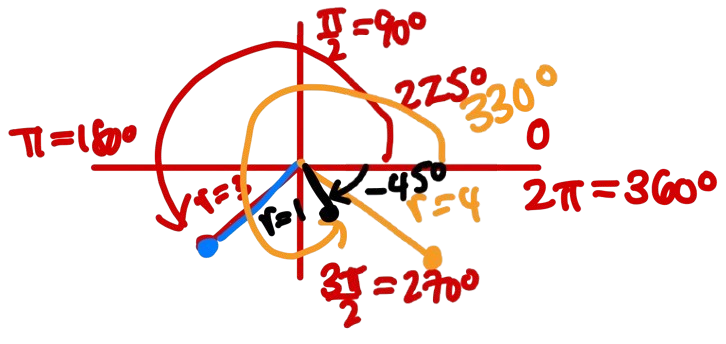
\includegraphics[width=\textwidth]{plot points example.png}
            \caption{Polar Coordinates Plot and ``Trajectories''}
            \label{fig:image2}
        \end{minipage}
    \end{figure}    
\end{solutionbox}
\end{examplebox}

\begin{tipbox}
    Ensure to label points clearly on the polar grid, and verify angle conversions and reflections for accuracy.
\end{tipbox}

\subsection*{Example: Converting from Polar Coordinates to Cartesian Coordinates}
\addcontentsline{toc}{subsection}{Example: Converting from Polar Coordinates to Cartesian Coordinates}

\begin{examplebox}
Find the \textbf{rectangular coordinates} of the point \( p \) with polar coordinates \( (6, \frac{\pi}{3}) \).

\begin{solutionbox}
To convert from polar to Cartesian coordinates, use:
\[
    x = r \cos \theta, \quad y = r \sin \theta
\]

Substitute \( r = 6 \) and \( \theta = \frac{\pi}{3} \):
\[
    x = 6 \cos\left(\frac{\pi}{3}\right) = 6 \cdot \frac{1}{2} = 3, \quad
    y = 6 \sin\left(\frac{\pi}{3}\right) = 6 \cdot \frac{\sqrt{3}}{2} = 3\sqrt{3}.
\]

Thus, the Cartesian coordinates are:
\[
    (x, y) = (3, 3\sqrt{3}).
\]

\begin{answerbox}
The rectangular coordinates are \( (3, 3\sqrt{3}) \).
\end{answerbox}
\end{solutionbox}
\end{examplebox}

\section*{Converting from Cartesian Coordinates to Polar Coordinates}
\begin{examplebox}
Find the \textbf{polar coordinates} of the point \( p \) with rectangular coordinates \( (-2, 2\sqrt{3}) \).

\begin{solutionbox}
To find the polar coordinates, use:
\[
    r^2 = x^2 + y^2, \quad \tan(\theta) = \frac{y}{x}.
\]

\textbf{Step 1: Solve for \( r \):}
\[
    r^2 = (-2)^2 + (2\sqrt{3})^2 = 4 + 12 = 16 \implies r = 4.
\]

\textbf{Step 2: Solve for \( \theta \):}
\[
    \tan(\theta) = \frac{y}{x} = \frac{2\sqrt{3}}{-2} = -\sqrt{3}.
\]

The point \( (-2, 2\sqrt{3}) \) lies in Quadrant II. The reference angle for \( \tan^{-1}(\sqrt{3}) \) is \( \frac{\pi}{3} \). Thus:
\[
    \theta = \pi - \frac{\pi}{3} = \frac{2\pi}{3}.
\]

\begin{tipbox}
    Alternatively, for a negative angle:
    \[
        \theta = -\frac{\pi}{3}, \quad \text{adjust to Quadrant II: } -\frac{\pi}{3} + \pi = \frac{2\pi}{3}.
    \]
\end{tipbox}

Thus, \( (r, \theta) = (4, \frac{2\pi}{3}) \).

\begin{answerbox}
The polar coordinates are \( (4, \dfrac{2\pi}{3}) \) or \( (4, 120^\circ) \).
\end{answerbox}
\end{solutionbox}
\end{examplebox}

\begin{notebox}
    To enhance material understanding, make use of graphing websites (e.g. Desmos, Geogebra) or software whenever possible. Focus especially on mastering how to plot lines and circles, as these are fundamental for MAT232.
\end{notebox}
\section*{Polar Curves}
\begin{examplebox}
Consider \( r = f(\theta) \). Sketch the following functions: 
\begin{enumerate}[label=(\alph*)]
    \item \( r = 1 \)
    \item \( \theta = \frac{\pi}{4} \)
    \item \( r = \theta, \quad \theta \geq 0 \)
    \item \( r = \sin(\theta) \)
    \item \( r = \cos(2\theta) \)
\end{enumerate}
\end{examplebox}

\subsection*{(a) \( r = 1 \)}
\begin{solutionbox}
Here, \( r = 1 \), and \( \theta \) can take any value. 

This means the point is always at a distance of \( 1 \) from the origin, regardless of the angle \( \theta \). Hence, the graph is a \textbf{circle} with radius \( 1 \), centred at the origin.

\begin{remarkbox}
    \textbf{\underline{Cartesian Conversion}} \\
    From the polar equation:
    \[
    x^2 + y^2 = r^2 = 1
    \]
    This confirms the equation of a unit circle in Cartesian coordinates.
\end{remarkbox}
\begin{figure}[H]
    \centering
    
\includegraphics[width=0.35\textwidth]{sample_image.jpg}
    \caption{Sample image illustrating the concept.}
    \label{fig:sample_image}
\end{figure}
\end{solutionbox}

\subsection*{(b) \( \theta = \dfrac{\pi}{4} \)}
\begin{solutionbox}
Here, \( \theta = \dfrac{\pi}{4} \), and \( r \) can take any value. 

This represents all points that lie along the line passing through the origin at an angle of \( \frac{\pi}{4} \) (or \( 45^\circ \)) with the positive \( x \)-axis. The graph is a straight line through the origin.

\begin{remarkbox}
    \textbf{\underline{Cartesian Conversion}} \\
    In polar coordinates:
    \[
    \tan(\theta) = \frac{y}{x}
    \]
    Substituting \( \theta = \frac{\pi}{4} \), we get:
    \[
    \tan\left(\frac{\pi}{4}\right) = 1 \quad \Rightarrow \quad \frac{\pi}{4} = \tan^{-1}\left(1\right) = \tan^{-1}\left(\frac{y}{x}\right) \quad \Rightarrow \quad 1 = \frac{y}{x} \quad \Rightarrow \quad y = x
    \]
    Thus, the Cartesian equation is \( y = x \).
\end{remarkbox}
\begin{figure}[H]
    \centering
    
\includegraphics[width=0.35\textwidth]{sample_image.jpg}
    \caption{Sample image illustrating the concept.}
    \label{fig:sample_image}
\end{figure}
\end{solutionbox}

\subsection*{(c) \( r = \theta, \quad \theta \geq 0 \)}
\begin{solutionbox}
Here, \( r \) increases as \( \theta \) increases. This creates a spiral that starts at the origin and winds outward as \( \theta \) grows. 

\begin{remarkbox}
    \textbf{\underline{Illustration}} \\
    Create a table of values to plot key points:
    \[
    \begin{array}{c|c}
    \theta & r \\
    \hline
    0 & 0 \\
    \frac{\pi}{6} & \frac{\pi}{6} \approx 0.52 \\
    \frac{\pi}{4} & \frac{\pi}{4} \approx 0.79 \\
    \frac{\pi}{3} & \frac{\pi}{3} \approx 1.05 \\
    \frac{\pi}{2} & \frac{\pi}{2} \approx 1.57 \\
    \end{array}
        \]
    \begin{notebox}
    Using \( x = r \cos\theta \) and \( y = r \sin\theta \), compute \( x \) and \( y \) for each point in the table above to visualize the curve in Cartesian coordinates.
    \end{notebox}
\end{remarkbox}
\begin{figure}[H]
    \centering
    
\includegraphics[width=0.35\textwidth]{sample_image.jpg}
    \caption{Sample image illustrating the concept.}
    \label{fig:sample_image}
\end{figure}
\end{solutionbox}

\subsection*{(d) \( r = \sin(\theta) \)}
\begin{solutionbox}
Here, \( r = \sin(\theta) \). Since \( \sin(\theta) \) oscillates between \( 0 \) and \( 1 \), the graph forms a \textbf{cardioid}.

\textbf{\underline{Table of Values}}
\[
\begin{array}{c|c|c|c|c|c|c}
\theta & 0 & \frac{\pi}{6} & \frac{\pi}{4} & \frac{\pi}{3} & \frac{\pi}{2} & \pi \\
\hline
r & 0 & \frac{1}{2} & \frac{\sqrt{2}}{2} & \frac{\sqrt{3}}{2} & 1 & 0 \\
\end{array}
\]

\textbf{\underline{Cartesian Conversion}} \\
To express the equation in Cartesian form:
\[
x = r \cos\theta, \quad y = r \sin\theta
\]
Eliminating \( r \), substitute \( r = \sin\theta \):
\[
r = \frac{y}{r} \quad \Rightarrow \quad r^2 = y
\]
Using \( r^2 = x^2 + y^2 \), we get:
\[
x^2 + y^2 = y
\]
Complete the square for \( y \):
\[
x^2 + \left(y - \frac{1}{2}\right)^2 = \frac{1}{4}
\]
This represents a circle centred at \( \left(0, \frac{1}{2}\right) \) with radius \( \frac{1}{2} \).

\begin{figure}[H]
    \centering
    
\includegraphics[width=0.35\textwidth]{sample_image.jpg}
    \caption{The graph of \( r = \sin(\theta) \).}
    \label{fig:cardioid_graph}
\end{figure}
The graph is a cardioid, touching the origin and looping around the point \( \left(0, \frac{1}{2}\right) \).
\end{solutionbox}

\begin{exercisebox}
    Try sketching the curve:
    \[
        r = \cos\theta
    \]
    under the same context as the previous questions.
    
    \begin{solutionbox}
    Here, \( r = \cos\theta \). Since \( \cos\theta \) oscillates between \( -1 \) and \( 1 \), the graph will form a \textbf{limacon} with an inner loop.
    
    \textbf{\underline{Table of Values}}
    To visualize the curve, create a table of key points:
    \[
    \begin{array}{c|c}
    \theta & r \\
    \hline
    0 & 1 \\
    \frac{\pi}{3} & \frac{1}{2} \\
    \frac{\pi}{2} & 0 \\
    \frac{2\pi}{3} & -\frac{1}{2} \\
    \pi & -1 \\
    \end{array}
    \]
    
    \begin{notebox}
        Plot the points in the table and connect them smoothly to form the graph. Note that for negative \( r \), the points are plotted in the opposite direction from the origin.
    \end{notebox}
    
    \textbf{\underline{Cartesian Conversion}}
    Substitute \( r = \cos\theta \) into the Cartesian equations:
    \[
    x = r \cos\theta \quad \text{and} \quad y = r \sin\theta
    \]
    Substituting \( r = \sqrt{x^2 + y^2} \) and eliminating \( r \), we derive:
    \[
    x^2 + y^2 = x
    \]
    Complete the square for \( x \):
    \[
    (x - \frac{1}{2})^2 + y^2 = \frac{1}{4}
    \]
    This represents a circle with centre \( (\frac{1}{2}, 0) \) and radius \( \frac{1}{2} \).
    
    \begin{figure}[H]
        \centering
        
\includegraphics[width=0.35\textwidth]{sample_image.jpg}
        \caption{Sample image illustrating the concept.}
        \label{fig:sample_image}
    \end{figure}

    The graph of \( r = \cos\theta \) is a limacon with an inner loop, and its Cartesian equivalent is the circle described above.
    \end{solutionbox}
\end{exercisebox}    

\section*{The Derivative of a Polar Curve}
\subsection*{Tangents to Polar Curves}
\begin{definitionbox}
\begin{notebox}
Recall that polar curves are defined by:
\[
    r = f(\theta)
\]
\end{notebox}
\[
    x = r\cos\theta = f(\theta) \cos\theta
\]
\[
    y = r\sin\theta = f(\theta) \sin\theta
\]
\begin{intuitionbox}
The goal is to have everything on \( x \) depend on \textbf{one} parameter. \\
\\
Do the exact same thing on \( y \).
\end{intuitionbox}

So, 
\[
    \dfrac{dy}{dx} = \dfrac{\dfrac{dy}{d\theta}}{\frac{dx}{\dfrac{d}{\theta}}}.
\]
We want require \( \frac{dx}{d\theta} \neq 0 \).

So\dots
\[
    \frac{dy}{dx} = \frac{\frac{dy}{d\theta}}{\frac{dx}{d\theta}}
\]
\[
    = \dfrac{\frac{df(\theta)}{d\theta} \sin\theta + \cos\theta f(\theta)}{\frac{df(\theta)}{d\theta} \cos\theta - \sin\theta f(\theta)}
\]
So,
\[
    \frac{dy}{dx} = \frac{\frac{dy}{d\theta}}{\frac{dx}{d\theta}} = \dfrac{\frac{dr}{d\theta} \sin\theta + r \cos\theta}{\frac{dr}{d\theta} \cos\theta - r \sin\theta}
\]
(subbed \( r \) in for \( f(\theta) \)).
\underline
\\
{Conclusion:}
\begin{itemize}
    \item Horizontal Tangents: \( \frac{dy}{d\theta} = 0, \quad \frac{dx}{d\theta} \neq 0 \)
    \item Vertical Tangents: \( \frac{dx}{d\theta} = 0, \quad \frac{dy}{d\theta} \neq 0 \)
    \item Singular Points (discard; we will not be doing further analysis for this case in MAT232): \( \frac{dy}{d\theta} = \frac{dx}{d\theta} = 0 \)
\end{itemize}

\end{definitionbox}

\section*{Examples}
\begin{examplebox}
Find the \textbf{vertical tangent} angles of the polar curve \( r = 1 - \cos\theta, \quad 0 \leq \theta \leq \pi \).
\begin{solutionbox}
Recall that \( \frac{dr}{d\theta} = \sin\theta \).

Obtain the first derivative:
\[
    \frac{dy}{dx} = ...
\]

\textbf{self-note: prof is going way too fast; finish the notes according to your camera roll later! the good thing is that you didn't actually miss any sections! fulfilling incomplete sections is just a matter of reviewing and comparing to the pictures taken of the prof's projected live notes!}

\begin{answerbox}
The vertical tangents are located at \( x = \{ \frac{\pi}{3}, \pi \} \).
\end{answerbox}
\end{solutionbox}

\begin{figure}[H]
    \centering
    
\includegraphics[width=0.35\textwidth]{sample_image.jpg}
    \caption{Sample image illustrating the concept.}
    \label{fig:sample_image}
\end{figure}

\end{examplebox}

\section*{Next Week: Vector Week}
\begin{theorembox}
\begin{itemize}
    \item Circle: \( x^2 + y^2 = r ^2 \).
    \item Generic form for a circle centered at \( (h, k) \): \( (x - h)^2 + (y - k)^2 = r^2 \)
\end{itemize}

\begin{figure}[H]
    \centering
    
\includegraphics[width=0.35\textwidth]{sample_image1.jpg}
    \caption{Graphical representation of the theorem.}
    \label{fig:sample_image1}
\end{figure}

\end{theorembox}

\begin{examplebox}
Sketch \( x^2 + y^2 - 2x = 10 \).

\begin{solutionbox}
Recall how to complete the square:
\[
    x^2 - 2x + 1 + y^2 = 10 + 1
\]
\underline{Step \#1:} \( -\frac{2}{2} = -1 \); \\
\underline{Step \#2:} \( (-1)^2 = 1 \) 
\textbf{self-note: complete this below} 
\end{solutionbox}
\end{examplebox}

\end{document}
